\documentclass[%
portrait,paperwidth=841mm,paperheight=1180mm,%
%landscape,
%a0paper,
margin=2cm,
fontscale=0.32
%fontscale=0.29
]{baposter}

\usepackage{environ}

\NewEnviron{headerblock}[2]{\headerbox{#1}{#2}{\BODY}}

\usepackage{marvosym,url,siunitx,paralist}
\usepackage{amsmath,amssymb,booktabs,dsfont,comment,epstopdf,multirow}
\usepackage{etoolbox}
\robustify\bfseries % requires etoolbox
\newcommand{\minitab}[2][l]{\begin{tabular}{#1}#2\end{tabular}}

\usetikzlibrary{intersections,decorations.pathreplacing,fit,calc,3d,positioning,shapes.geometric,matrix}
\pgfdeclarelayer{background}
\pgfsetlayers{background,main}

\newcommand{\vect}[1]{\vec{#1}}
\newcommand{\mus}{\vec{\mu}}
\newcommand{\data}{\mathcal{D}}
\newcommand{\given}{\mid}
\DeclareMathOperator{\sigm}{sigm}
\DeclareMathOperator{\conj}{conj}
\DeclareMathOperator{\fft}{fft}
\DeclareMathOperator{\ifft}{ifft}
\newcommand{\R}{\ensuremath{\mathds{R}}}
\newcommand{\Q}{\ensuremath{\mathds{Q}}}
\newcommand{\N}{\ensuremath{\mathds{N}}}
\newcommand{\E}{\ensuremath{\mathds{E}}}
\newcommand{\F}{\ensuremath{\mathcal{F}}}
\newcommand{\Norm}{\ensuremath{\mathcal{N}}}

\renewcommand*\sfdefault{uop}
\newcommand{\spanA}{2}
\newcommand{\spanB}{2}

%\selectcolormodel{cmyk}

\begin{document}

%\definecolor{ubcblue}{cmyk}{0.392, 0.352, 0.051, 0.267}
\definecolor{ubcblue}{HTML}{002145}
\definecolor{ubcgraya}{HTML}{5E869F}
\definecolor{ubcgrayb}{HTML}{2F5D7C}
\definecolor{ubcgrayc}{HTML}{98B2C3}
\definecolor{ubcgrayd}{HTML}{C3D0DB}
\definecolor{ubcgrayf}{HTML}{B7C9D3}

\newcommand{\alert}[1]{\textbf{\textcolor{ubcblue}{#1}}}
\newcommand{\minisection}[1]{\textcolor{ubcblue}{\large\textbf{%
\tikz \fill[ubcblue] (0,0)-- ++(90:0.25)-- ++(-30:0.25)--cycle; #1}}\\[0.5em]}
\setdefaultleftmargin{1em}{}{}{}{.5em}{.5em}
\setlength{\plitemsep}{4.0pt plus 1.0pt minus 1.0pt}
\setlength{\pltopsep}{8.0pt plus 1.0pt minus 4.0pt}
\setlength{\plpartopsep}{2.0pt plus 1.0pt minus 1.0pt}

\renewcommand*\descriptionlabel[1]{%
\hspace\labelsep\bfseries\textcolor{ubcblue}{#1}}

\sffamily

%\background{
%\begin{tikzpicture}[remember picture,overlay]%
%  %\draw (current page.north west)+(-2em,2em) node[anchor=north west]
%  %{\includegraphics[height=1.1\textheight]{background}};
%  \fill[ubcgray!20!white] (current page.north west) rectangle (current
%  page.south east);
%  \end{tikzpicture}
%}

\newcommand{\inst}[1]{$^{#1}$}

\begin{poster}{
  %grid=false,
  %eyecatcher=false,
  columns=4,
  background=shadetb,
  bgColorOne=white,
  bgColorTwo=white,
  %bgColorTwo=ubcgrayf,
  headershade=plain,
  headershape=roundedright,
  headerColorOne=ubcblue,
  headerColorTwo=ubcblue,
  borderColor=ubcblue,
  boxshade=none,
  textborder=faded,
  headerborder=open,
  headerFontColor=white,
  headerfont=\scshape\Large,
  linewidth=1pt,
  %headerheight=0.135\textheight,
  %colspacing=1.25em
  headerheight=0.19\textwidth,
  colspacing=1.25em
}
%%% Eye Catcher %%%
{

\includegraphics[width=0.17\textwidth]{images/Logo_MICCAI15}
}
%%% Title %%%
{
% Manifold\hspace{0.5ex}Learning\hspace{0.5ex}of\hspace{0.5ex}Brain\hspace{0.5ex}MRIs\\
% by\hspace{0.5ex}Deep\hspace{0.5ex}Learning~~\vspace{0.5em}
Deep Convolutional Encoder Networks for\\ Multiple Sclerosis Lesion
Segmentation\vspace{0.5em} }
%%% Authors %%%
{
%Tom Brosch$^1$ and Roger Tam$^2$, MS/MRI Research Group, UBC,
%Vancouver\\[0.65ex]
%$^1$\texttt{tombr@msmri.medicine.ubc.ca}, $^2$\texttt{roger.tam@ubc.ca}
\Large
Tom Brosch\inst{1,4},
Youngjin Yoo\inst{1,4},
Lisa Y.W. Tang\inst{4},
David K.B. Li\inst{2,4},\\
Anthony Traboulsee\inst{3,4}, and
Roger Tam\inst{2,4}\\[0.65ex]
\normalsize \inst{1}Department of Electrical and Computer Engineering,
UBC\quad \inst{2}Department of Radiology, UBC\\[0.65ex]
\inst{3}Division of Neurology, UBC\quad
\inst{4}MS/MRI Research Group, University of British Columbia, Vancouver, Canada
%\\[0.65ex]
}
%%% Logo %%%
{
\begin{tabular}{c}
\\

\includegraphics[height=0.08\textwidth]{images/s4b282c}\\
\addlinespace

\includegraphics[height=0.04\textwidth]{images/msmri_simple}
\end{tabular}
}

%%%%%%%%%%%%%%%%%%%%%%%%%
% Footer
%%%%%%%%%%%%%%%%%%%%%%%%%

% \begin{headerblock}{Acknowledgement}{above=bottom, column=0,name=acknowledgement}
% 
% This work was supported by the Natural Sciences and Engineering Research Council
% of Canada and the Milan and Maureen Ilich Foundation.
% 
% \end{headerblock}

%%%%%%%%%%%%%%%%%%%%%%%%%
% Introduction
%%%%%%%%%%%%%%%%%%%%%%%%%

\begin{headerblock}{Introduction}{row=0, column=0, name=introduction,span=1}
\begin{compactitem}
\item Multiple sclerosis (MS) is an inflammatory and demyelinating disease of
the central nervous system, and is characterized by the formation of lesions,
primarily visible in the white matter on conventional MRIs.
\item Imaging biomarkers based on the delineation of lesions, such as lesion
load and lesion count, have established their importance for assessing disease
progression and treatment effect.
% \item However, lesions vary greatly in size, shape,
% intensity and location, which makes their automatic and accurate segmentation
% challenging.
\item We propose a new method for segmenting MS lesions that processes entire
MRI volumes through a neural network
%with a novel objective function
to automatically learn features tuned for lesion segmentation. 
\end{compactitem}
\end{headerblock}

%%%%%%%%%%%%%%%%%%%%%%%%%
% Contributions
%%%%%%%%%%%%%%%%%%%%%%%%%

\begin{headerblock}{Contributions}{row=0, column=1, name=contributions,
span=1}
\begin{compactitem}
\item Our network processes entire volumes instead of patches, which removes the
need to select representative patches, eliminates redundant calculations where
patches overlap, and therefore scales up more efficiently with image resolution.
\item Our approach combines feature learning and segmentation in a single model,
which allows for the automatic learning of features that are tuned towards lesion
segmentation.
\item We propose a new objective function based on a weighted combination of
sensitivity and specificity, designed to deal with unbalanced classes, as is the
case for lesions, which typically comprise less than \SI{1}{\percent} of the
image voxels.
\end{compactitem}
\end{headerblock}

%%%%%%%%%%%%%%%%%%%%%%%%%
% Overview
%%%%%%%%%%%%%%%%%%%%%%%%%

% \begin{headerblock}{Overview}{row=0, column=1, span=1}
% \begin{compactdesc}
%   \item[Data set:] 474 T1-weighted, T2-weighted, and PD-weighted MRIs of
%   secondary progressive MS patients with a resolution of \num{256x256x50} voxels
%  and a voxel size of \SI{0.937x0.937x3.000}{\milli\meter}
%  \item[Pre-processing:] Brain extraction, intensity normalization, background
%  cropping, lesion segmentation, affine registration to ICBM 152 nonlinear atlas
%  template image
%  \item[Morphology model:] a model that aims to find patterns of morphological changes in deformation
% fields
% \item[Lesion model:] a model that aims to find patterns in the spatial
% distribution of lesions
% \item[Joint model:] a joint model that aims to find concurring deformation and
% lesion distribution patterns
% \end{compactdesc}
% \end{headerblock}

%%%%%%%%%%%%%%%%%%%%%%%
% Method 
%%%%%%%%%%%%%%%%%%%%%%%
\begin{headerblock}{Method}{below=contributions, name=method, span=2}
\begin{compactitem}
\item The task of segmenting MS lesions is defined as finding a function $s$
that maps multi-modal images $I$, e.g., $I = (I_\text{FLAIR}, I_\text{T1},
I_\text{T2})$, to corresponding lesion masks $S$.
\item Given a training set $(I_n,S_n)$, finding $s$ is modeled as an
optimization problem of the following form
\begin{equation}
\hat{s} = \arg \min_{s \in \mathcal{S}} \sum_n E(S_n, s(I_n))
\label{eq:segprob}
\end{equation}
where $\mathcal{S}$ is the set of possible segmentation functions, and $E$ is an
error measure.
%\end{compactitem}
%\end{headerblock}
%\begin{headerblock}{Method (continued)}{row=0, column=1, name=method2}
%\begin{compactitem}
\item The set of possible segmentation functions, $\mathcal{S}$, is modeled by
the following 3-layer convolutional encoder network:
\end{compactitem}
\begin{center}
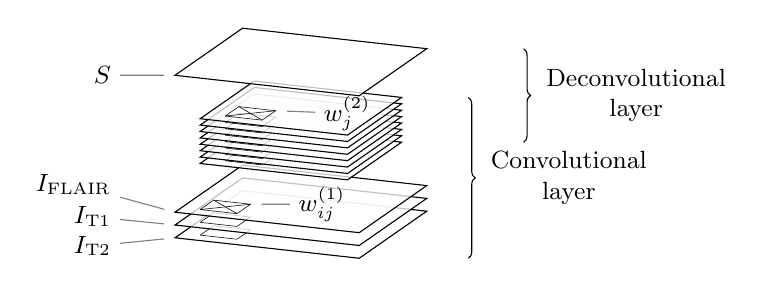
\begin{tikzpicture}[%
scale=0.65,
x  = {(0.9cm,-0.1cm)},
y  = {(0.33cm,0.23cm)},
z  = {(0cm,1cm)}]

\tikzstyle{every node}=[font=\small, inner sep=3pt, align=center]
\tikzstyle{every pin}=[align=center,fill=white]
\tikzstyle{dbnlabel}=[font=\sffamily\normalsize]

\tikzstyle{image}=[fill=white, fill opacity=0.75]
\tikzstyle{pinline}=[thin, gray]
\tikzstyle{kernelline}=[very thin]


%%%%%%%%%%%%%%%%%         
% INPUT LAYER
%%%%%%%%%%%%%%%%%

\foreach \x in {1, ..., 3} {
\begin{scope}[canvas is xy plane at z=0.25*\x]
\draw[image] (-2,-2) coordinate (A\x) -- (2,-2)
coordinate (B\x) -- (2,2) coordinate (C\x) -- (-2,2) -- cycle;

\draw[kernelline] 
      (-1.6, -1.6) \ifnum\x=3 \else -- +(0, 0, 0.25) +(0,0) \fi
   -- (-0.8, -1.6) \ifnum\x=3 \else -- +(0, 0, 0.25) +(0,0) \fi
   -- (-0.8, -0.8) \ifnum\x=3 \else -- +(0, 0, 0.25) +(0,0) \fi
   -- (-1.6, -0.8) \ifnum\x=3 \else -- +(0, 0, 0.25) +(0,0) \fi
   -- (-1.6, -1.6);
\ifnum\x=3
\draw[kernelline] (-1.6, -1.6) -- (-1.2, -1.2, 0.9);
\draw[kernelline] (-1.6, -0.8) -- (-1.2, -1.2, 0.9);
\draw[kernelline] (-0.8, -0.8) coordinate(c3) -- (-1.2, -1.2, 0.9);
\draw[kernelline] (-0.8, -1.6) -- (-1.2, -1.2, 0.9);
\fi 

\end{scope}
}

\node[xshift=-0.7cm, yshift=10pt, left] (flair) at (A3) {$I_\text{FLAIR}$};
\node[xshift=-0.7cm, yshift=3pt, left] (t1w) at (A2) {$I_\text{T1}$}; 
\node[xshift=-0.7cm, yshift=-3pt, left] (t2w) at (A1) {$I_\text{T2}$};
% \node[xshift=-0.7cm, yshift=-10pt, left] (prior) at (A0) {$I_\text{prior}$};

\draw[pinline, shorten >=4pt] (flair) -- (A3);
\draw[pinline, shorten >=4pt] (t1w) -- (A2);
\draw[pinline, shorten >=4pt] (t2w) -- (A1);
% \draw[pinline, shorten >=4pt] (prior) -- (A0);

% \draw[decorate,decoration={brace,raise=15pt,mirror}] (C1) --
% node[right=20pt] {$x^{(1)}_i$} (C3);

\node[xshift=0.5cm, right] (weights) at (c3) {$w^{(1)}_{ij}$};
\draw[pinline, shorten >=4pt] (weights) -- (c3);

%%%%%%%%%%%%%%%%%         
% HIDDEN LAYER
%%%%%%%%%%%%%%%%%

\foreach \x in {0, ..., 7} {
\begin{scope}[canvas is xy plane at z=0.125*\x+1.65]
\draw[image] (-1.6,-1.6) -- (1.6,-1.6)
-- (1.6,1.6) coordinate (G\x) -- (-1.6,1.6) -- cycle;

\draw[kernelline]
      (-1.2, -1.2) \ifnum\x=7 \else -- +(0, 0, 0.125) +(0,0) \fi
   -- (-0.4, -1.2) \ifnum\x=7 \else -- +(0, 0, 0.125) +(0,0) \fi
   -- (-0.4, -0.4) \ifnum\x=7 \else -- +(0, 0, 0.125) +(0,0) \fi
   -- (-1.2, -0.4) \ifnum\x=7 \else -- +(0, 0, 0.125) +(0,0) \fi
   -- (-1.2, -1.2);
\ifnum\x=7
\draw[kernelline] (-1.2, -1.2) -- (-0.8, -0.8, 0.9);
\draw[kernelline] (-1.2, -0.4) -- (-0.8, -0.8, 0.9);
\draw[kernelline] (-0.4, -0.4) coordinate (g7) -- (-0.8, -0.8, 0.9);
\draw[kernelline] (-0.4, -1.2) -- (-0.8, -0.8, 0.9);
\fi 

\end{scope}
}

% \draw[decorate,decoration={brace,raise=15pt,mirror}] (G0-|C1) --
% node[right=20pt] {$x^{(2)}_j = y^{(1)}_j$} (G7-|C1);

\node[xshift=0.5cm, yshift=-1pt, right] (weights2) at (g7) {$w^{(2)}_{j}$};
\draw[pinline, shorten >=4pt] (weights2) -- (g7);


%%%%%%%%%%%%%%%%%         
% OUTPUT LAYER
%%%%%%%%%%%%%%%%%

\begin{scope}[canvas is xy plane at z=3.425]
\draw[image] (-2,-2) coordinate (A) -- (2,-2)
-- (2,2) coordinate (C) -- (-2,2) -- cycle;
\end{scope}

\node[xshift=-0.7cm, left] (lesion) at (A) {$S$};
\draw[pinline, shorten >=4pt] (lesion) -- (A);

% \node[xshift=0.7cm, right] (y2) at (C) {$y^{(2)}$};
% \draw[pinline, shorten <=4pt] (C) -- (y2);

\draw[decorate,decoration={brace,raise=15pt,mirror}] (B1-|C) --
node[right=20pt] {Convolutional\\ layer} (G7-|C1);

\draw[decorate,decoration={brace,raise=35pt,mirror}] (G0-|C1) --
node[right=40pt] {Deconvolutional\\ layer} (C);

\end{tikzpicture}
\end{center}
% %\end{headerblock}
% 
% %\begin{headerblock}{Method (continued)}{row=0, column=1,name=method}
\begin{compactitem}
\item The input layer is composed of the image voxels of different
modalities.
\item The convolutional layer extracts features from the input layer at
each voxel location.
\item The deconvolutional layer uses the extracted features to predict a lesion
mask and thereby classify each voxel of the image in a single operation.
\item The error measure, $E$, is a weighted sum of the mean squared
difference of the lesion voxels (sensitivity) and non-lesion voxels
(specificity), reformulated to be error terms.
\begin{equation}
E = r\frac{\textstyle\sum_{\vect{p}} \left(S(\vect{p}) -
y^{(2)}(\vect{p})\right)^2 S(\vect{p})}{\textstyle\sum_{\vect{p}} S(\vect{p})}
+(1-r)\frac{\textstyle\sum_{\vect{p}} \left(S(\vect{p}) -
y^{(2)}(\vect{p})\right)^2 \big(1 - S(\vect{p})\big)}{%
\textstyle\sum_{\vect{p}}\big(1 - S(\vect{p})\big)}
\end{equation}
\end{compactitem}
% % \begin{multline}
% % E = r\frac{\textstyle\sum_{\vect{p}} \left(S(\vect{p}) -
% % y^{(2)}(\vect{p})\right)^2 S(\vect{p})}{\textstyle\sum_{\vect{p}} S(\vect{p})}\\
% %   +
% % (1-r)\frac{\textstyle\sum_{\vect{p}} \left(S(\vect{p}) -
% % y^{(2)}(\vect{p})\right)^2 \big(1 - S(\vect{p})\big)}{%
% % \textstyle\sum_{\vect{p}}\big(1 - S(\vect{p})\big)}
% % \end{multline}
\vspace{1.5em}
\end{headerblock}

%%%%%%%%%%%%%%%%%%%%%%%%%
% Evaluation
%%%%%%%%%%%%%%%%%%%%%%%%%

\begin{headerblock}{Evaluation}{row=0, column=2, name=evaluation, span=2}

\minisection{Evaluation on Public Data}
\begin{compactdesc}
\item[Dataset] FLAIR, T1-, and T2-weighted MRIs of the
20 publicly available labeled cases from the MS lesion segmentation challenge
2008 \cite{styner20083d}.
\item[Pre-processing] Downsampled from the original isotropic voxel
size of \SI{0.5}{\cubic\milli\metre} to an isotropic voxel size of
\SI{1.0}{\cubic\milli\metre}
\end{compactdesc}
\begin{compactitem}
\item Example segmentations of our method for three different subjects.
\item Our method performed well and consistently despite the
large contrast differences seen between the first two rows.
\item In the third row, our method also segmented regions that have similar
contrast, although these regions had not been identified as lesions by the
manual rater.
\end{compactitem}

% \vspace{0.5em}
\def\MRIwidth{0.13\textwidth}
\begin{center}
\begin{tikzpicture}[every node/.append style={font=\footnotesize}]
\tikzstyle{leftlabel}=[rotate=90, align=center,above]

\matrix [matrix of nodes, ampersand replacement=\&, nodes={anchor=center, inner
sep=1.5pt}] {
\&[4pt] FLAIR \& T1w \& T2w \& Gold \& CEN \\[2pt]
\node[leftlabel] {CHB\,07\\DSC\,=\,\SI{60.58}{\percent}}; \&
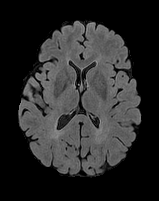
\includegraphics[width=\MRIwidth]{figures/CHB07-FLAIR-s88} \&
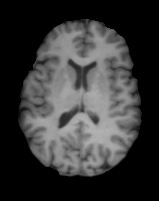
\includegraphics[width=\MRIwidth]{figures/CHB07-T1w-s88} \&
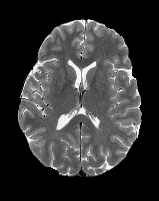
\includegraphics[width=\MRIwidth]{figures/CHB07-T2w-s88} \&
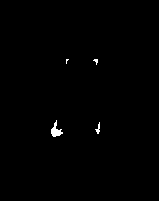
\includegraphics[width=\MRIwidth]{figures/CHB07-gold-s88} \&
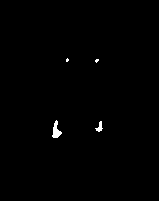
\includegraphics[width=\MRIwidth]{figures/CHB07-pred-s88} \\
\node[leftlabel] {CHB\,07\\DSC\,=\,\SI{60.58}{\percent}}; \&
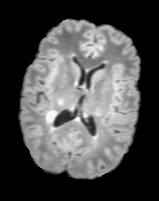
\includegraphics[width=\MRIwidth]{figures/CHB04-FLAIR-s85} \&
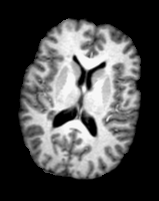
\includegraphics[width=\MRIwidth]{figures/CHB04-T1w-s85} \&
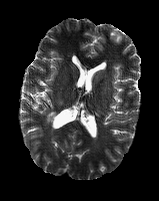
\includegraphics[width=\MRIwidth]{figures/CHB04-T2w-s85} \&
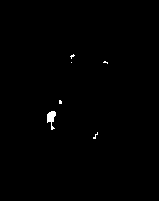
\includegraphics[width=\MRIwidth]{figures/CHB04-gold-s85} \&

\includegraphics[width=\MRIwidth]{figures/CHB04-pred-s85} \\
\node[leftlabel] {UNC\,09\\DSC\,=\,\SI{9.01}{\percent}}; \&
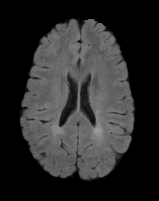
\includegraphics[width=\MRIwidth]{figures/UNC09-FLAIR-s89} \&
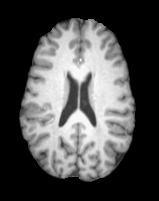
\includegraphics[width=\MRIwidth]{figures/UNC09-T1w-s89} \&
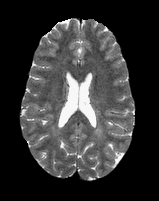
\includegraphics[width=\MRIwidth]{figures/UNC09-T2w-s89} \&

\includegraphics[width=\MRIwidth]{figures/UNC09-gold-s89} \&

\includegraphics[width=\MRIwidth]{figures/UNC09-pred-s89} \\
};
\end{tikzpicture}
\end{center}
%\end{headerblock}

%\begin{headerblock}{Evaluation (continued)}{row=0, column=2, name=evaluation}
\begin{compactitem}
\item Comparison of our method with state-of-the-art lesion segmentation
methods in terms of mean TPR, PPV, and DSC.
\end{compactitem}
\begin{center}
\def\tabspace{12pt}
\begin{tabular}{l%
@{\hspace{\tabspace}}S[table-format=2.2]
@{\hspace{\tabspace}}S[table-format=2.2]
@{\hspace{\tabspace}}S[table-format=2.2]
}
\toprule
Method & {TPR} & {PPV} & {DSC} \\ 
\midrule
Souplet et al. [1] & 20.65 & 30.00 & {---} \\ 
Weiss et al. [2] & 33.00 & 36.85 & 29.05 \\ 
Geremia et al. [3] & 39.85 & 40.35 & {---}  \\
Our method & 39.71 & 41.38 & 35.52 \\
\bottomrule
\end{tabular}
\end{center}

\minisection{Evaluation on a Large Data Set from an MS Clinical Trial}

\begin{compactdesc}
\item[Dataset] The T2- and PD-weighted MRIs of 500 subjects acquired from 45
different scanning were sites split equally into training and test sets.
\item[Pre-processing] Rigid intra-subject registration, brain extraction,
intensity normalization, and background cropping.
%(\SI{0.937x0.937x3.000}{\milli\metre})  
\end{compactdesc}
\begin{compactitem}
\item Comparison of DSC scores calculated on the training and test sets for
varying numbers of training samples.
\item Approximately 100 samples are required to train the model without
overfitting.
\end{compactitem}
\begin{center}
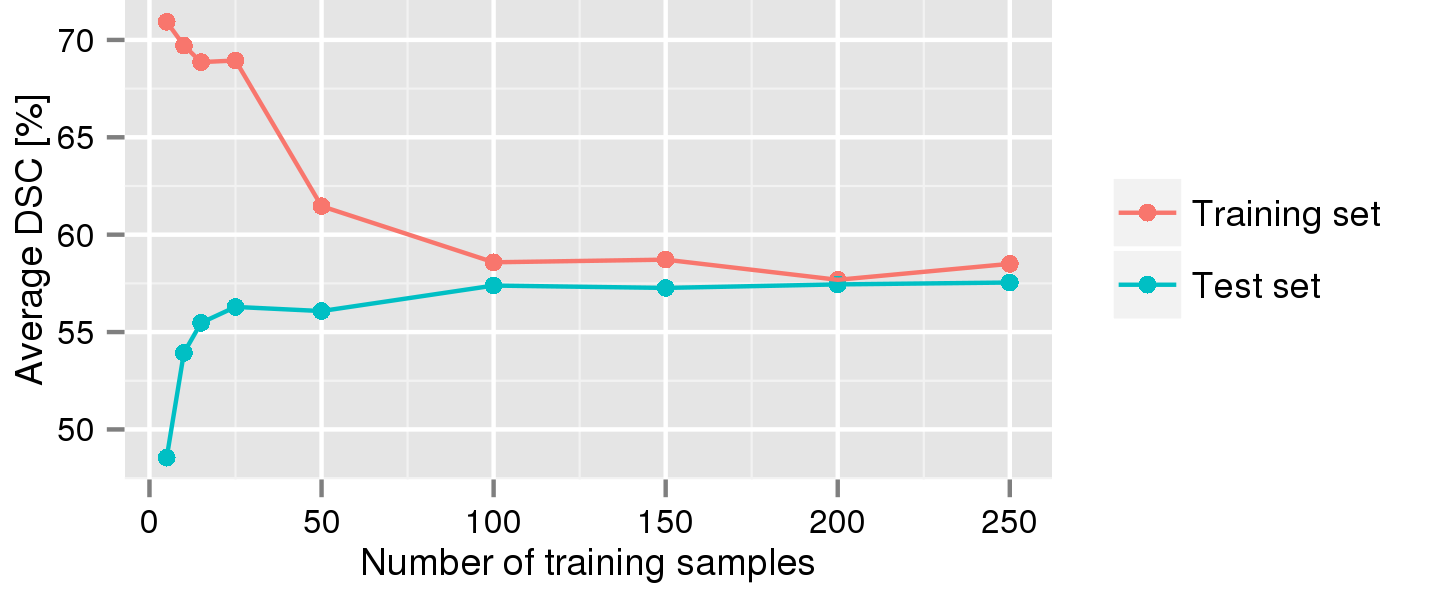
\includegraphics[width=0.9\textwidth]{figures/train_count}
\end{center}
\end{headerblock}

% TODO: Put some of these statements into the main text and make figures a
% little bit smaller to make everything fit.

% \begin{headerblock}{Conclusions}{below=evaluation, column=2,
% name=conclusions,above=bottom, span=1}
% \begin{compactitem} 
%   \item Our method performs comparably to the best methods reported on the MS
% lesion segmentation challenge 2008 data set.
%   \item Segmentation performance can be greatly improved by having a
%   representative data set.
% \end{compactitem} 
% \end{headerblock}

 %\begin{headerblock}{Video}{below=method, column=1, above=bottom, span=1}
 %\end{headerblock}


%\normalsize 
\begin{headerblock}{Contact Information and Video}{%below=acknowledgement,
column=0, span=2, above=bottom, name=contact}
% \begin{tabular}{@{}c@{\, }ll}
\begin{tabular}{@{}clc@{\hspace{5pt}}c}
  \Letter & \texttt{brosch.tom@gmail.com} &
  \multirow{4}{*}{\hspace{2em}Video:} &
  \multirow{4}{*}{\includegraphics[width=0.15\textwidth]{images/qrcode}}
  \\
  \Mundus & \url{tbrosch.blogspot.com} \\
  \includegraphics[width=0.8em]{images/linkedin} &
  %\url{/in/tombrosch} \\
  \url{linkedin.com/in/tombrosch} \\
  \tikz \node[fill=black,text=white,inner sep=1pt, rounded
  corners=1pt]{ \includegraphics[height=0.6em]{images/RG_white_Logo}};
  %& \url{/profile/Tom_Brosch} \\
  & \url{researchgate.net/profile/Tom_Brosch} \\
  %& \multicolumn{1}{c}{\includegraphics[width=0.5\textwidth]{figures/contact}}
\end{tabular}
%\Letter\ \texttt{tombr@msmri.medicine.ubc.ca}\quad\Mundus{}
%\url{http://tbrosch.blogspot.com/}
\end{headerblock}

\begin{headerblock}{Acknowledgement}{column=0, span=2,
name=acknowledgement,above=contact,below=method}
This work was supported by the Natural Sciences and
Engineering Research Council of Canada and the Milan and Maureen Ilich Foundation.
\end{headerblock}

\begin{headerblock}{References}{%below=evaluation,
column=2,span=2,above=bottom}
\small
\begin{compactenum}[{[1]}]
\item[{[1]}] Souplet et al., ``An automatic segmentation
of T2-FLAIR multiple sclerosis lesions.'' In: MIDAS Journal -- MICCAI 2008
Workshop (2008)
\item[{[2]}] Weiss et al., ``Multiple sclerosis lesion segmentation using
dictionary learning and sparse coding.'' In: MICCAI 2013, Part I. LNCS, vol. 8149, pp. 735--742.
\item[{[3]}] Geremia et al., ``Spatial decision forests for MS lesion
segmentation in multi-channel MR images.'' In: MICCAI 2010, Part I. LNCS, vol. 6361, pp.
111--118.
\end{compactenum}
% [1] Souplet et al., ``An automatic segmentation
% of T2-FLAIR multiple sclerosis lesions.'' In: MIDAS Journal -- MICCAI 2008
% Workshop (2008)
% \\[0.25em]
% [2] Weiss et al., ``Multiple sclerosis lesion segmentation using dictionary
% learning and sparse coding.'' In: MICCAI 2013, Part I. LNCS, vol. 8149, pp. 735--742.
% \\[0.25em]
% [3] Geremia et al., ``Spatial decision forests for MS lesion segmentation in
% multi-channel MR images.'' In: MICCAI 2010, Part I. LNCS, vol. 6361, pp.
% 111--118.
\end{headerblock}

% TODO: add references
% TODO: Put a picture of me on the poster so people can find me at the
% conference if I'm not at my poster

% \headerbox{Contact}{name=contact,below=acknowledge}{
% Please contact us via e-mail:
% \begin{compactitem}
%   \item Tom Brosch: \texttt{tombr@msmri.medicine.ubc.ca}
%   \item Roger Tam: \texttt{roger.tam@ubc.ca}
% \end{compactitem}
% }

\end{poster}

\end{document}